\documentclass[preview]{standalone}

\usepackage{amsmath}
\usepackage{amssymb}
\usepackage{stellar}
\usepackage{definitions}
\usepackage{tikz}

\usetikzlibrary{arrows.meta,positioning,decorations.markings,backgrounds}

\tikzset{
    every node/.style={font=\footnotesize},
}

\begin{document}

\genpage{false}

\begin{snippet}{dipole-field-lines-illustration}
    \begin{center}
    % https://tex.stackexchange.com/questions/248967/draw-dipole-field-lines
    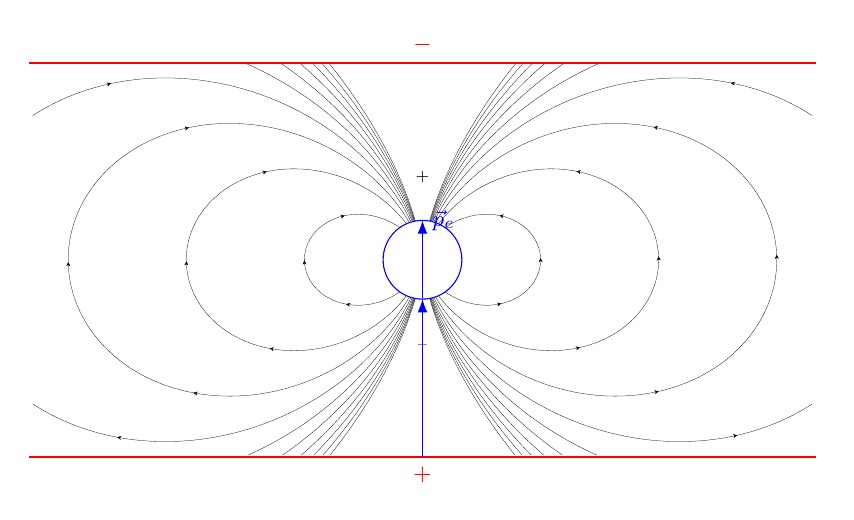
\begin{tikzpicture}[-, scale=2.5]
    \def\my{.5mm}

    \draw [thick, red] (-2,-1) -- node [below] {+} (2,-1) node (v3) {};
    \draw [thick, red] (-2,1) -- node [above] {$-$}  (2,1) ;

    \node[draw=blue, fill=white, circle, ,minimum size=1cm, inner sep=0, outer sep=0] (circ) at (0,0) {};
    \draw [-{Latex},blue] (0,-1) -- (circ.south);
    \node [below] (v2) at (0,.5) {\tiny +};
    \node [above] (v1) at (0,-.5) {\tiny  --};
    \draw [-{Latex}, blue] (0,-.2) -- (0,.2) node [right] {$\vec p_{e}$};

    %\path[clip] (-2,0) -- (2,0) -- (2,2) -- (-2,2) -- cycle;
    \begin{scope}[scale=.3,on background layer]
    \clip[scale=3.3] (-2,-1) rectangle (2,1);
    \foreach \a [count=\b] in {1,2,3,4,5,6,7,8,9,10}{
        \draw[domain=0:6.3,samples=500, line width=.1pt, decoration={markings,%
            mark=at position 0.1 with {\arrow{Stealth[width=\my,length=\my]}},
            mark=at position 0.4 with {\arrowreversed{Stealth[width=\my,length=\my]}},
            mark=at position 0.5 with {\arrowreversed{Stealth[width=\my,length=\my]}},
            mark=at position 0.6 with {\arrowreversed{Stealth[width=\my,length=\my]}},
            mark=at position 0.9 with {\arrow{Stealth[width=\my,length=\my]}},
            mark=at position 1 with {\arrow{Stealth[width=\my,length=\my]}},}, postaction=decorate] plot (xy polar cs:angle=\x r,radius={\a+\b*cos(2*\x r)});
    }
    \end{scope}
    \end{tikzpicture}
    \end{center}
\end{snippet}

\end{document}